%-------------------------------------------------------%
%       CPP- Programming Intro                          %
%-------------------------------------------------------%


\documentclass[english,xcolor=pdftex,dvipsnames,aspectratio=169]{beamer} 

\usepackage{babel}
\usepackage[utf8]{inputenc}
\usepackage[T1]{fontenc}
\usepackage{amsfonts,amsmath,amssymb}
\usepackage{wrapfig}
\usepackage{color,colortbl}
\usepackage{upquote}
\usepackage{ifthen}

\definecolor{pblue}{RGB}{45,106,148}
\definecolor{pdarkblue}{RGB}{35,71,100}
\definecolor{plightblue}{RGB}{90,159,212}
\definecolor{pyellow}{RGB}{255,212,59}
\definecolor{pdarkyellow}{RGB}{255,188,41}
\definecolor{orange}{RGB}{255,165,0}
\definecolor{plightyellow}{RGB}{255,232,115}
\definecolor{pdarkgrey}{RGB}{100,100,100}
\definecolor{pgrey}{RGB}{153,153,153}
\definecolor{plightgrey}{RGB}{233,233,233}
\definecolor{plightgrey2}{RGB}{247,247,247}
\definecolor{pnavy}{RGB}{0,0,170}
\definecolor{BrickRed}{RGB}{150,22,11}
\definecolor{BlueViolet}{RGB}{138, 43, 226}
\definecolor{PineGreen}{RGB}{0, 51, 0}
\definecolor{light-gray}{gray}{0.95}

\definecolor{UniRot}{RGB}{193,0,42}
\definecolor{UniDunkelGrau}{RGB}{99,99,99}
\definecolor{UniHellGrau}{RGB}{172,172,172}

\definecolor{UrlColor}{rgb}{0,0.08,0.45}
\definecolor{tcA}{rgb}{0.627451,0.627451,0.643137}


\usetheme{CambridgeUS} % Pittsburgh, CambridgeUS
\usecolortheme{beaver} %wolverine | crane | beaver | seahorse
\useinnertheme{rounded} 
\useoutertheme{default}
\usefonttheme{default}
%\setbeamercovered{transparent}
\setbeamertemplate{footline}[frame number]
\setbeamersize{text margin left=0.5cm, text margin right=0.5cm}

\setbeamercolor{structure}{fg=UniRot}% to modify  immediately all palettes
\setbeamercolor{title}{fg=UniRot}
\setbeamercolor{title in head/foot}{fg=UniRot}
\setbeamercolor{block title}{fg=white,bg=orange}
\setbeamercolor{block title alerted}{fg=white,bg=UniRot}
\setbeamercolor{block title example}{fg=white,bg=PineGreen!80}


% enables two line cols in tabular envs
\newcommand{\specialcell}[2][c]{%
  \begin{tabular}[#1]{@{}c@{}}#2\end{tabular}}

\usepackage{tikz}
\usetikzlibrary{arrows,shapes,snakes,backgrounds,positioning,shadows,decorations,trees}

\usepackage{smartdiagram}
\usesmartdiagramlibrary{additions}
\usepackage{tikzpeople}

\addtobeamertemplate{footline}{}{%
\begin{tikzpicture}[remember picture,overlay]
\node[anchor=south west,yshift=2pt] at (current page.south west) {
\includegraphics[height=0.8cm]{images/logos/nhr_sw3_k50.png} 
\includegraphics[height=0.8cm]{images/logos/DRA_LogoNoText.png}};
\end{tikzpicture}}

\usepackage[tikz]{bclogo}
\newcommand{\task}[2][Over to you]{\begin{bclogo}[arrondi=0.1,logo=\bcoutil]{#1} #2 \end{bclogo}}
\newcommand{\docs}[2][Documentation]{\begin{bclogo}[arrondi=0.1,logo=\bcbook]{#1} #2 \end{bclogo}}
\newcommand{\hint}[2][Hint]{\begin{bclogo}[arrondi=0.1,logo=\bcinfo]{#1} #2 \end{bclogo}}
\newcommand{\warning}[2][Warning]{\begin{bclogo}[arrondi=0.1,logo=\bcattention]{#1} #2 \end{bclogo}}
% ``d/Definition'' is already defined ;-)
\newcommand{\explanation}[2][Definition]{\begin{bclogo}[arrondi=0.1,logo=\bcplume]{#1} #2 \end{bclogo}}
\newcommand{\question}[2][Question]{\begin{bclogo}[arrondi=0.1,logo=\bcquestion]{#1} #2 \end{bclogo}}

\usepackage{marvosym}
\usepackage[load-configurations=binary,binary-units=true]{siunitx}
\usepackage{todonotes}
\usepackage{multicol}

\usepackage{hhline}
\usepackage[labelformat=empty]{caption}

\usepackage{times}

\usepackage{dirtree,float} % for directory tree listings
\usepackage[nodisplayskipstretch]{setspace}

% will decrease the font size for one frame
\newcommand\Fontvi{\fontsize{6}{7.2}\selectfont}

\usepackage{verbatim}
\usepackage{fancyvrb,cprotect} % to enable # in verbatim mode
\usepackage{listings}

\newcommand\YAMLcolonstyle{\color{red}\bfseries}
\newcommand\YAMLkeystyle{\color{black}\bfseries}
\newcommand\YAMLvaluestyle{\color{blue}\mdseries}
\newcommand\YAMLemphasisstyle{\color{red}\bfseries}

\makeatletter
\newcommand\language@yaml{yaml}
\expandafter\expandafter\expandafter\lstdefinelanguage
\expandafter{\language@yaml}
{
	keywords={true,false,null,y,n},
	keywordstyle=\color{darkgray}\bfseries,
	basicstyle=\YAMLkeystyle,
	sensitive=false,
	comment=[l]{\#},
	morecomment=[s]{/*}{*/},
	commentstyle=\color{purple}\ttfamily,
	stringstyle=\YAMLvaluestyle\ttfamily,
	moredelim=[l][\color{orange}]{\&},
	moredelim=[l][\color{magenta}]{*},
	moredelim=**[il][\YAMLcolonstyle{:}\YAMLvaluestyle]{:},
	morestring=[b]',
	morestring=[b]",
	literate=
	{---}{{\ProcessThreeDashes}}3
	{>}{{\textcolor{red}\textgreater}}1     
	{|}{{\textcolor{red}\textbar}}1 
	{\ -\ }{{\mdseries\ -\ }}3
	{@}{{\makeatletter @ \makeatother}}1
	{!}{{\YAMLemphasisstyle}}1,
	keepspaces=true,
	escapechar=\%,
	alsoletter={ },
	extendedchars=false,
	breaklines=true,
	breakatwhitespace=true,
	breakindent=0pt,
	postbreak=\raisebox{0ex}[0ex][0ex]{\ensuremath{\hookrightarrow\space}},
	linewidth=\textwidth,
}
\makeatother

\newcommand\ProcessThreeDashes{\llap{\color{cyan}\mdseries-{-}-}}

\lstloadlanguages{              %
  % Python,                       %
   bash,                         %
  C++,
  yaml                           %
}

% Listing for Shell
\lstdefinestyle{Shell}
{
  language=Bash,
  basicstyle=\ttfamily\small,
  showstringspaces=false,
  % frame=single,
  % framerule=0.4pt,
  rulecolor=\color{pgrey},
  backgroundcolor=\color{plightgrey2},
  stringstyle=\color{BrickRed},
  keywordstyle=\color{BlueViolet},
  commentstyle=\color{PineGreen}\bfseries,
  identifierstyle=\color{black},
  emph={[10]\$,>>>}, emphstyle={[10]\color{pblue}},
  moredelim=**[is][\bfseries\color{red}]{@}{@}
}


% Listing for C++
\lstdefinestyle{C++}
{                               %
  language=C++,                 %
  basicstyle=\scriptsize,       %
  showstringspaces=false,       %
  stepnumber=5,                 %
  numberstyle=\tiny,            %
  numbersep=5pt,                %
  showspaces=false,             
  % frame=single,                 
  % framerule=0.2pt,              
  rulecolor=\color{pgrey},      
  backgroundcolor=\color{plightgrey2}, 
  stringstyle=\color{magenta},        
  keywordstyle=\color{blue},           
  commentstyle=\color{PineGreen}\bfseries, 
  identifierstyle={},                      
  emph={[10]this}, emphstyle={[10]\color{pblue}}, 
  emph={[11]auto}, emphstyle={[11]\color{pblue}},
  morekeywords={type},
  moredelim=[is][\bfseries\color{red}]{@}{@}     
}

%default shell listings:
\lstdefinestyle{Shell}
{
	language=Bash,
	basicstyle=\ttfamily\small,
	showstringspaces=false,
	frame=single,
	framerule=0.4pt,
	rulecolor=\color{pgrey},
	backgroundcolor=\color{plightgrey2},
	stringstyle=\color{BrickRed},
	keywordstyle=\color{BlueViolet},
	commentstyle=\color{PineGreen}\bfseries,
	identifierstyle=\color{black},
	emph={[10]\$,>>>}, emphstyle={[10]\color{pblue}},
	moredelim=**[is][\bfseries\color{red}]{@}{@},
	literate={\\@}{{\makeatletter @ \makeatother}}1
}

\makeatletter
\newcommand\applyCurrentFontsize
{%
	% we first save the current fontsize, baseline-skip,
	% and listings' basicstyle
	\let\f@sizeS@ved\f@size%
	\let\f@baselineskipS@ved\f@baselineskip%
	\let\basicstyleS@ved\lst@basicstyle%
	% we now change the fontsize of listings' basicstyle
	\renewcommand\lst@basicstyle%
	{%
		\basicstyleS@ved%
		\fontsize{\f@sizeS@ved}{\f@baselineskipS@ved}%
		\selectfont%
	}%
}
\makeatother

\newcommand{\altverb}[2][{}]{\colorbox{plightgrey}{\applyCurrentFontsize \lstinline[language={#1}]{#2}}}

\newcommand{\CC}{C\nolinebreak\hspace{-0.05em}\raisebox{0.1em}{++}}

\newcommand{\bibtex}{\textsc{Bib}\TeX}


%%% https://tex.stackexchange.com/questions/99316/symbol-for-external-links
\newcommand{\LinkSymbol}{%
  \tikz[x=1.2ex, y=1.2ex, baseline=-0.05ex]{% 
    \begin{scope}[x=1ex, y=1ex]
      \clip (-0.1,-0.1) 
      --++ (-0, 1.2) 
      --++ (0.6, 0) 
      --++ (0, -0.6) 
      --++ (0.6, 0) 
      --++ (0, -1);
      \path[draw, 
      line width = 0.5, 
      rounded corners=0.5] 
      (0,0) rectangle (1,1);
    \end{scope}
    \path[draw, line width = 0.5] (0.5, 0.5) 
    -- (1, 1);
    \path[draw, line width = 0.5] (0.6, 1) 
    -- (1, 1) -- (1, 0.6);
  }
}
\usepackage{nameref}
\newcommand{\lhref}[2]{\href{#1}{#2\,\LinkSymbol}}

\setbeamertemplate{section page}
{
    \begin{centering}
    \begin{beamercolorbox}[sep=12pt,center]{part title}
    \usebeamerfont{section title}\insertsection\par
    \end{beamercolorbox}
    \end{centering}
}


\newcounter{handson}
\setcounter{handson}{1}
\newcounter{preframe_handson}
\setcounter{preframe_handson}{1}
\newcommand{\HandsOn}[1]{Hands On \Roman{handson} -- #1 \addtocounter{handson}{1}}

\newcounter{interlude}
\setcounter{interlude}{1}
\newcounter{preframe_interlude}
\setcounter{preframe_interlude}{1}
\newcommand{\Interlude}[1]{Interlude \Roman{interlude} -- #1 \addtocounter{interlude}{1}}

\newcounter{advertisements}
\setcounter{advertisements}{1}
\newcounter{preframe_advertisements}
\setcounter{preframe_advertisements}{1}
\newcommand{\Advertisement}[1]{Advertisement \Roman{advertisements} -- #1 \addtocounter{advertisements}{1}}

%%%% shortcuts for uniform appearance of common strings %%%%
\newcommand{\slurm}{\textsc{slurm}~}
\makeatletter
\newcommand{\rmnum}[1]{\romannumeral #1}
\newcommand{\Rmnum}[1]{\expandafter\@slowromancap\romannumeral #1@}
\makeatother
\usepackage{xspace}
\newcommand{\mogon}{\textsc{mogon}\xspace}
\newcommand{\mogonI}{\textsc{mogon}\,\Rmnum{1}\xspace}
\newcommand{\mogonII}{\textsc{mogon}\,\Rmnum{2}\xspace}

\setcounter{tocdepth}{1}

%--------------------%
% Meta-Info 
%--------------------%

\title[CI Course]{Continuous Integration} 
\subtitle{An Introduction}
\author[DRA]{Christian Meesters - DRA}
\institute{
\includegraphics[width=4cm]{images/logos/nhr_sw3_k50.png}
\includegraphics[width=2cm]{images/logos/DRA_LogoNoText.png}}
\date{\newline{\scriptsize Edition 1} -- \scriptsize 9.10.2025}
%\titlegraphic{\includegraphics[width=1.5cm,height=1.5cm]{Logo_klein}}

\definecolor{links}{HTML}{2A1B81}
\hypersetup{colorlinks,linkcolor=,urlcolor=links}

\graphicspath{{images/}}


%%%%%%%%%%%%%%%%%%%%%%%%%%%%%%%%%%%%%%%%%%%%%%%%%%%%%%%%%%%%%%%%%%%%%%%%%%%%%%%%
%%%%%%%%%%%%%%%%%%%%%%%%%%%%%%%%%%%%%%%%%%%%%%%%%%%%%%%%%%%%%%%%%%%%%%%%%%%%%%%%
\begin{document}
%%%%%%%%%%%%%%%%%%%%%%%%%%%%%%%%%%%%%%%%%%%%%%%%%%%%%%%%%%%%%%%%%%%%%%%%%%%%%%%%
%%%%%%%%%%%%%%%%%%%%%%%%%%%%%%%%%%%%%%%%%%%%%%%%%%%%%%%%%%%%%%%%%%%%%%%%%%%%%%%%






% For every picture that defines or uses external nodes, you'll have to
% apply the 'remember picture' style. To avoid some typing, we'll apply
% the style to all pictures.
\tikzstyle{every picture}+=[remember picture]
\tikzstyle{na} = [baseline=-.5ex]
\tikzstyle{ind} = [rectangle,   %
% drop shadow,                    %
draw=black, %thick,
rounded corners,                %
minimum width=0.5cm,            %
minimum height=0.4cm]

\tikzstyle{host} = [rectangle,  %
% drop shadow,                    %
draw=black, %thick,
rounded corners,                %
minimum width=7.8cm,            %
minimum height=1.1cm]



%%%% nicer typesetting the snakemake project
\newcommand{\Snakemake}{\mbox{
		\begingroup\normalfont
		
\includegraphics[height=1em]{logos/Snakemake.png}
		\textbf{Snakemake}
		\endgroup}}

% Passe captions an
\setbeamertemplate{caption}{\insertcaption}
\setbeamerfont{caption}{size=\footnotesize}
\setlength\abovecaptionskip{0pt}
\setlength\belowcaptionskip{0pt}

% Passe das Inhaltsverzeichnis an
\setbeamertemplate{section in toc}[square]

%%%%%%%%%%%%%%%%%%%%%%%%%%%%%%%%%%%%%%%%%%%%%%%%%%%%%%%%%%%%%%%%%%%%%%%%%%%%%%%%
% Gebe den aktuellen Pfad zu den Aufgaben und den Loesungen an !
% \newcommand{\pathtoexercise}[1]{\path{/project/hpckurs/cpp-intro/samples/#1}}
% \newcommand{\pathtosolution}[1]{\path{/project/hpckurs/cpp-intro/solutions/#1}}
% \newcommand{\pathtoexample}[1]{\path{/project/hpckurs/cpp-intro/examples/#1}}
\newcommand{\pathtoexercise}[1]{\path{code/samples/#1}}
\newcommand{\pathtosolution}[1]{\path{code/solutions/#1}}
\newcommand{\pathtoexample}[1]{\path{code/examples/#1}}
%%%%%%%%%%%%%%%%%%%%%%%%%%%%%%%%%%%%%%%%%%%%%%%%%%%%%%%%%%%%%%%%%%%%%%%%%%%%%%%%
% Und dies sind die Pfade zu den Bilder und Logos

%\newcommand{\pathtoimages}[1]{\path{../images/#1}}
\newcommand{\pathtologos}[1]{\path{../logos/#1}}



%%%%%%%%%%%%%%%%%%%%%%%%%%%%%%%%%%%%%%%%%%%%%%%%%%%%%%%%%%%%%%%%%%%%%%%%%%%%%%%%
\begin{frame}[plain] % plain erzeugt Titelseite ohne Kopf- und Fußzeile
  \titlepage
\end{frame}

%%%%%%%%%%%%%%%%%%%%%%%%%%%%%%%%%%%%%%%%%%%%%%%%%%%%%%%%%%%%%%%%%%%%%%%%%%%%%%%% 
\begin{frame}
  \frametitle{Outline}
  \begin{columns}[t]
    \begin{column}{.5\textwidth}
      \tableofcontents[sections={1-8}]
    \end{column}
    \begin{column}{.5\textwidth}
      \tableofcontents[sections={9-16}]
    \end{column}
  \end{columns}
\end{frame}

%%%%%%%%%%%%%%%%%%%%%%%%%%%%%%%%%%%%%%%%%%%%%%%%%%%%%%%%%%%%%%%%%%%%%%%%%%%%%%%%
\begin{frame}<handout:0>
	\frametitle{About Me}
	\begin{columns}
		\begin{column}{0.5\textwidth}
		   \begin{itemize}
		   	 \item PhD in Biophysics (Conformational Changes of BIG Protein Complexes studied with SAXS)
		   	 \item PostDoc in Genetic Epidemiology (first HPC Experience)
		   	 \item Detour in Industry
		   	 \item since 2014 LifeScience Support Specialist, HPC Group, Mainz, Germany
		   	 
		   \end{itemize}
		\end{column}
	    \begin{column}{0.5\textwidth}
	    	Social Media
	    	\begin{itemize}
	    		\item \lhref{https://fediscience.org/\@rupdecat}{Mastodon}
	    		\item \lhref{https://blogs.fediscience.org/rupture-de-catenaire/}{rupture de caténaire - Blog}
	    	\end{itemize}
    	    \pause
    	    Also:
    	    \begin{itemize}
    	    	\item various RSE roles, particularly: \Snakemake{}-Co-Maintainer \& the \slurm-plugin for \Snakemake
    	    \end{itemize}
	    \end{column}
	\end{columns}
\end{frame}

%%%%%%%%%%%%%%%%%%%%%%%%%%%%%%%%%%%%%%%%%%%%%%%%%%%%%%%%%%%%%%%%%%%%%%%%%%%%%%%%
\begin{frame}<handout:0>
	\frametitle{What about You?}
	\begin{question}[Who are you?]{
		Briefly, introduce yourself
		\begin{itemize}
			\item Name
			\item Scientific Subject (i.\,e. Computer Science, Physics, Life Science ...)
			\item RSE Role
		\end{itemize}}
	\end{question}
\end{frame}
%%%%%%%%%%%%%%%%%%%%%%%%%%%%%%%%%%%%%%%%%%%%%%%%%%%%%%%%%%%%%%%%%%%%%%%%%%%%%%%%
\section{About Continuous Integration}
{   
	\usebackgroundtemplate{
		\vbox to \paperheight{\vfil\hbox to \paperwidth{\hfil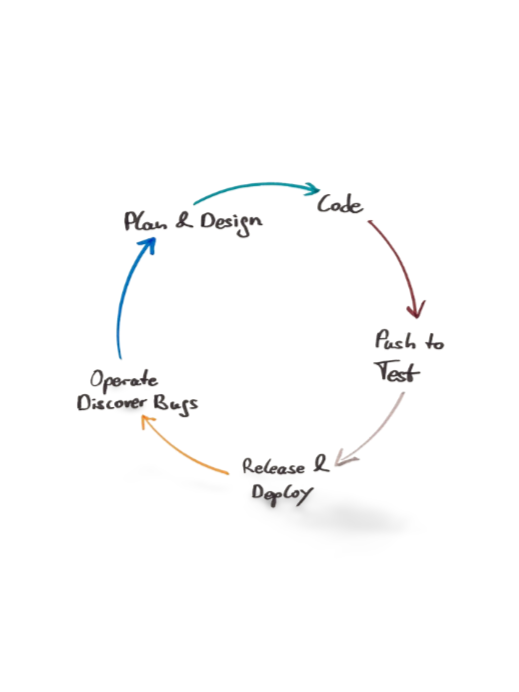
\includegraphics[height=\paperheight]{CI_enh.png}\hfil}\vfil}
		%https://www.flaticon.com/free-icon/decoration_2788716
		%<a href="https://www.flaticon.com/free-icons/decoration" title="decoration icons">Decoration icons created by Freepik - Flaticon</a>
		
	}
	\frame{
		\frametitle{The What \& Why}
		\begin{mdframed}[tikzsetting={draw=white,fill=white,fill opacity=0.8,
				line width=0pt},backgroundcolor=none,leftmargin=0,
			rightmargin=150,innertopmargin=4pt,roundcorner=10pt]
			\tableofcontents[currentsection,sections={1-6},hideothersubsections]
		\end{mdframed}
	}
}

%%%%%%%%%%%%%%%%%%%%%%%%%%%%%%%%%%%%%%%%%%%%%%%%%%%%%%%%%%%%%%%%%%%%%%%%%%%%%%%%
\begin{frame}
	\frametitle{The “Emotions”}
	\begin{columns}
		\begin{column}{0.5\textwidth}
			\centering 
			Idealized Software Development Cycle
			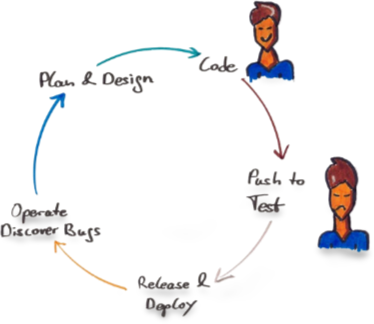
\includegraphics[width=0.8\textwidth]{CI_emotions_enh.png}
		\end{column}
		\begin{column}{0.5\textwidth}
			% A short introductory sentence (outside the list)
			What is Continuous Integration about?
			% The list with the *environment‑wide* overlay specification
			\begin{itemize}[<+->]
				\item We are passionate about coding \ldots
				\item But the TDD‑pill is hard to swallow
				\item Yet, needed for successful RSE projects.
			\end{itemize}
		\end{column}
	\end{columns}
\end{frame}

%%%%%%%%%%%%%%%%%%%%%%%%%%%%%%%%%%%%%%%%%%%%%%%%%%%%%%%%%%%%%%%%%%%%%%%%%%%%%%%%
\begin{frame}
	\frametitle{The “Background”}
	\begin{columns}
	    \begin{column}{0.5\textwidth}
			\centering 
			Idealized Software Development Cycle
			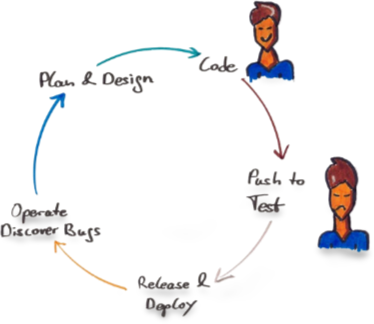
\includegraphics[width=0.8\textwidth]{CI_emotions_enh.png}
		\end{column}
		\begin{column}{0.5\textwidth}
			% A short introductory sentence (outside the list)
			We know \ldots
			% The list with the *environment‑wide* overlay specification
			\begin{itemize}[<+->]
				\item well tested  \ldots
				\item and actively maintained \ldots
			\end{itemize}
		    research software is used (and cited) more frequently
		    \pause
		    Also community building depends (in parts) on
		    \begin{itemize}[<+->]
		    	\item readable code
		    	\item and the knowing it is in good hands.
		    \end{itemize}
		\end{column}

	\end{columns}
\end{frame}

%%%%%%%%%%%%%%%%%%%%%%%%%%%%%%%%%%%%%%%%%%%%%%%%%%%%%%%%%%%%%%%%%%%%%%%%%%%%%%%%
\begin{frame}
	\frametitle{Which are the CI-Ingredients?}
	\begin{question}[What do you think?]
		{
		
\includegraphics[height=1.2em]{ingredients.jpg}
		What belongs to a CI Pipeline?
	}
	\end{question}
\end{frame}

%%%%%%%%%%%%%%%%%%%%%%%%%%%%%%%%%%%%%%%%%%%%%%%%%%%%%%%%%%%%%%%%%%%%%%%%%%%%%%%%
\begin{frame}
	\frametitle{Which are the CI-Constituents?}
	\begin{columns}
		\begin{column}{0.5\textwidth}
			\centering 
			Mandatory:
			\vfill
			\begin{itemize}[<+->]
				\item Version Control
				\item Package Management
				\item Automated Build Processes
				\item Automated Releases
			\end{itemize}
		\end{column}
		\begin{column}{0.5\textwidth}
			\centering
			Optional:
            \vfill

			\begin{itemize}[<+->]
			  \item Linting (Static Code Analysis)
			  \item for compiled languages: debug and release runs with difference compilers and settings, possibly checks for memory leaks.
			  \item Formatting (sometimes disliked)
			  \item Posting on Social Media
			\end{itemize}
		\end{column}	
	\end{columns}
\end{frame}

%%%%%%%%%%%%%%%%%%%%%%%%%%%%%%%%%%%%%%%%%%%%%%%%%%%%%%%%%%%%%%%%%%%%%%%%%%%%%%%%
\begin{frame}
	\frametitle{Our Current CI Options in RSE}
	\begin{columns}
		\begin{column}{0.4\textwidth}
			\centering 
			\only<1>{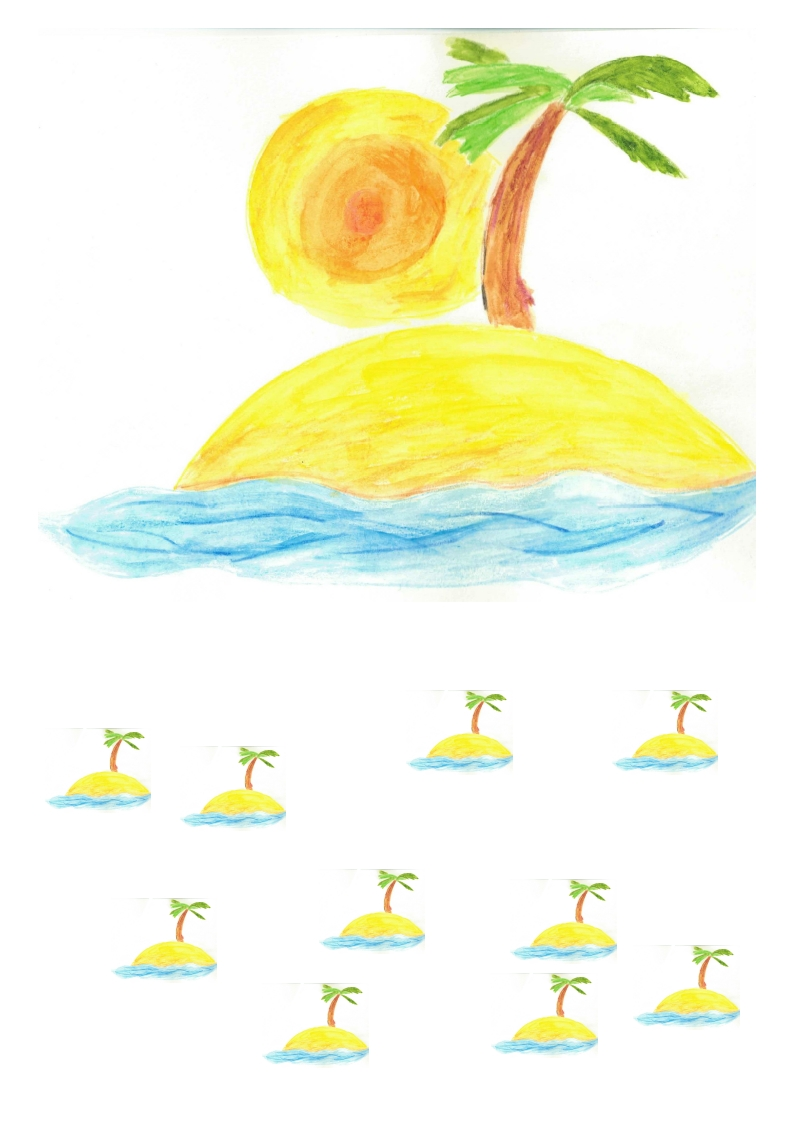
\includegraphics[width=0.8\textwidth]{Islands.jpg}}
			\only<2>{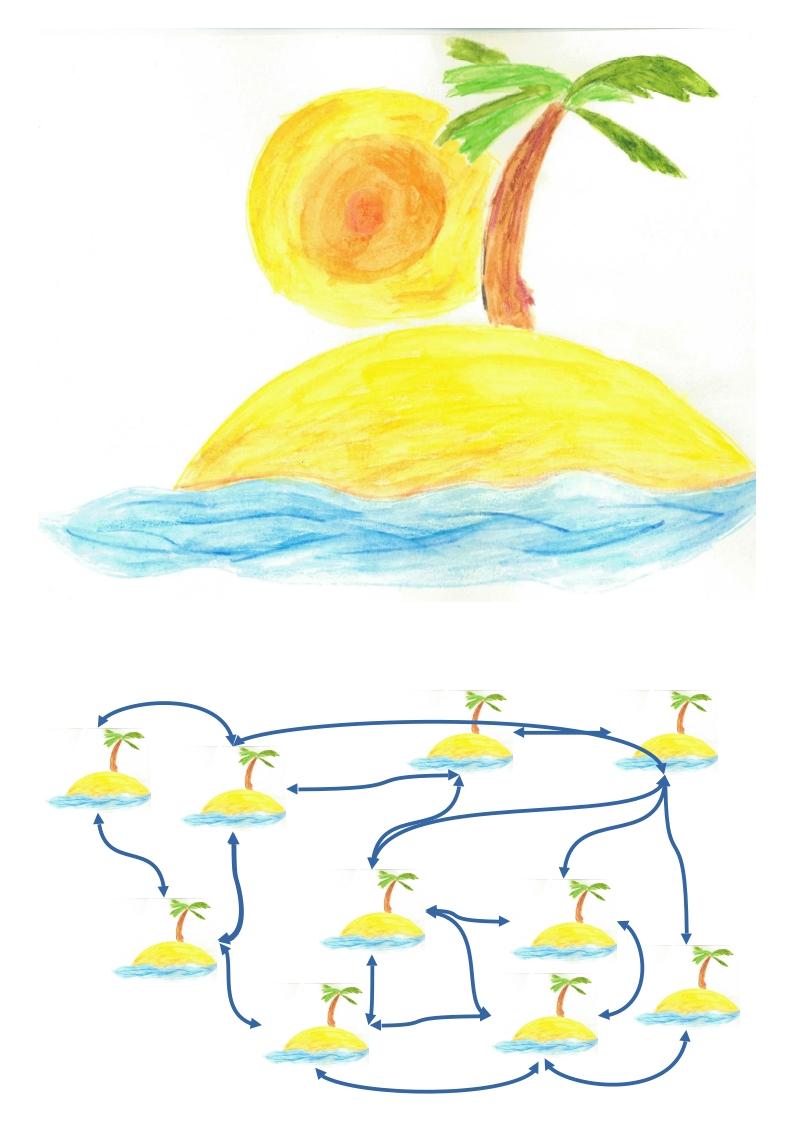
\includegraphics[width=0.8\textwidth]{Islands_connected.jpg}}
		\end{column}
		\begin{column}{0.6\textwidth}
			After cvs, svn, mecurial, etc. the RSE world settled for git -- close to 100 \% -- for source code management. Regarding CI, we have:
			\pause
			\begin{itemize}
				\item There is GitHub.com - the big beautiful island big enough for all, with all its cornucopia of features.
				\item Our institutions set on GitLab. Isolated. Good enough for interal projects.
				\only<3>{\item Perhaps, once ActivityPub is established for GitLab and Codeberg (Forgejo), we find ourselves in a different situation.}
			\end{itemize}
		\end{column}
	\end{columns}
\end{frame}

%%%%%%%%%%%%%%%%%%%%%%%%%%%%%%%%%%%%%%%%%%%%%%%%%%%%%%%%%%%%%%%%%%%%%%%%%%%%%%%%
\begin{frame}<handout:0>
	\frametitle{The Focus on GitHub}
	\begin{block}{This is why \ldots}
				\ldots we focus on GitHub, today. With bits of GitLab, too.\newline
		No Codeberg: The CI is with costs.\\
		This might change in future editions of this course.
	\end{block}
\end{frame}
	
%%%%%%%%%%%%%%%%%%%%%%%%%%%%%%%%%%%%%%%%%%%%%%%%%%%%%%%%%%%%%%%%%%%%%%%%%%%%%%%%
\section{Our Task}
{   
	\usebackgroundtemplate{
		\vbox to \paperheight{\vfil\hbox to \paperwidth{\hfil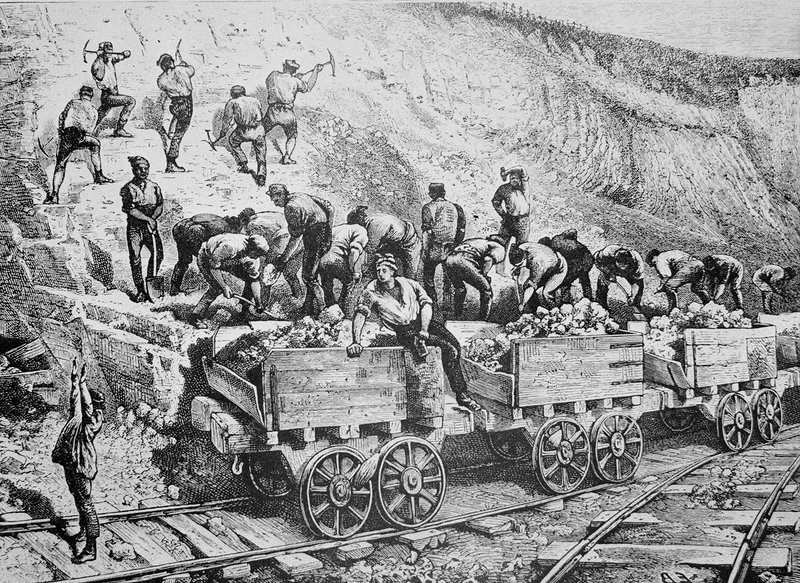
\includegraphics[height=\paperheight]{Railway_construction,_19th_century.jpg}\hfil}\vfil}
		%https://www.flaticon.com/free-icon/decoration_2788716
		%<a href="https://www.flaticon.com/free-icons/decoration" title="decoration icons">Decoration icons created by Freepik - Flaticon</a>
		
	}
	\frame{
		\frametitle{Let's get started}
		\begin{mdframed}[tikzsetting={draw=white,fill=white,fill opacity=0.8,
				line width=0pt},backgroundcolor=none,leftmargin=0,
			rightmargin=150,innertopmargin=4pt,roundcorner=10pt]
			\tableofcontents[currentsection,sections={1-6},hideothersubsections]
		\end{mdframed}
	}
}

%%%%%%%%%%%%%%%%%%%%%%%%%%%%%%%%%%%%%%%%%%%%%%%%%%%%%%%%%%%%%%%%%%%%%%%%%%%%%%%%
\begin{frame}
	\frametitle{Our Task \ldots}
	\ldots
	is simple. We are going to
	\begin{itemize}
		\item convert degrees of Fahrenheit into Celsius using $\circ\mathsf{C} = \frac{\circ\mathsf{F} - 32}{1.8}$
		\item estimate the value of $\pi$ by throwing darts in a circle.
	\end{itemize}
    Our code is broken and we fill see this using a CI pipeline!
    \pause
    \begin{question}[Is this too simple?]
    	{In real RSE, we are frequently dealing with little bugs, i.\,e. a wrong digit, a false memory access, etc.}
    \end{question}
\end{frame}

%%%%%%%%%%%%%%%%%%%%%%%%%%%%%%%%%%%%%%%%%%%%%%%%%%%%%%%%%%%%%%%%%%%%%%%%%%%%%%%%
\begin{frame}
	\frametitle{\HandsOn{Forking a Repository}}
	\begin{block}{Background}
		{Forking repos is the first step fixing a software, if you are not a team member of that project.}
	\end{block}
	\pause
	\begin{columns}
		\begin{column}{0.5\textwidth}
			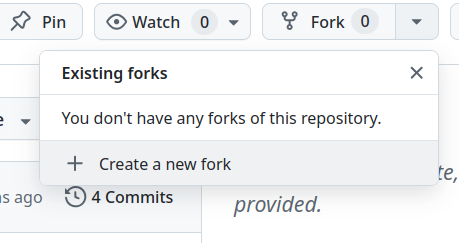
\includegraphics[width=0.9\textwidth]{fork.png}
		\end{column}
		\begin{column}{0.5\textwidth}
			Please fork the repo \url{https://github.com/cmeesters/ci-exercises}.
		\end{column}
	\end{columns}
\end{frame}

%%%%%%%%%%%%%%%%%%%%%%%%%%%%%%%%%%%%%%%%%%%%%%%%%%%%%%%%%%%%%%%%%%%%%%%%%%%%%%%%
\begin{frame}[fragile]
	\frametitle{\HandsOn{Cloning a Repository}}
	So, you just forked a repo as your "own" fork. This is how you get it locally.
	\begin{lstlisting}[language=Bash, style=Shell,escapeinside={(*}{*)}]
$ git clone git(*@*)github.com:<username>/ci-exercises
	\end{lstlisting}
    \begin{columns}
    	\begin{column}{0.5\textwidth}
    		\centering
    		\begin{minipage}[t]{0.8\textwidth}
    			\setstretch{0.1}
    			{\tiny \DTsetlength{0.2em}{1em}{0.2em}{0.4pt}{.6pt}
    				\dirtree{%
    					.1 {CMakeLists.txt}.
    					.1 {pyproject.toml}.
    					.1 {environment.yaml}.
    					.1 {src}.
    					.2 {converter.py}.
    					.2 {\ldots}.
    					.2 {pi\_estimator.cpp}.
    					.2 {tests}.
    					.3 {test\_converter.py}.
    					.3 {test\_pi\_estimator.cpp}.
    			}}
    		\end{minipage}
    	\end{column}
        \begin{column}{0.5\textwidth}
        	\begin{hint}
        		{From no on, we assume that you are working in the \altverb{ci-exercises} directory.}
        	\end{hint}
        \end{column}
    \end{columns}
    Afterwards your repo should look like (plus some files):
   

\end{frame}


%%%%%%%%%%%%%%%%%%%%%%%%%%%%%%%%%%%%%%%%%%%%%%%%%%%%%%%%%%%%%%%%%%%%%%%%%%%%%%%%
\begin{frame}<handout:0>[fragile]
	\frametitle{Activating the Conda Environment}
	\begin{lstlisting}[language=Bash, style=Shell]
$ conda activate ci-exercises
    \end{lstlisting}
\end{frame}

%%%%%%%%%%%%%%%%%%%%%%%%%%%%%%%%%%%%%%%%%%%%%%%%%%%%%%%%%%%%%%%%%%%%%%%%%%%%%%%%
\begin{frame}[fragile]
	\frametitle{Running Tests locally (Python)}
	\begin{warning}[The Importance of local Testing]
		{By running tests locally, you can avoid being surprised during the CI run and can fix code \emph{before} pushing to the git origin.}
	\end{warning}
    \pause
    \begin{lstlisting}[language=Bash, style=Shell]
$ # to test the python code
$ poetry run pytest tests/
$ # to produce a coverage report run
$ poetry run coverage run -m pytest tests/
$ poetry run coverage report
    \end{lstlisting}	
\end{frame}



%%%%%%%%%%%%%%%%%%%%%%%%%%%%%%%%%%%%%%%%%%%%%%%%%%%%%%%%%%%%%%%%%%%%%%%%%%%%%%%%
\begin{frame}
	\frametitle{\HandsOn{Something is broken \ldots}}
	\ldots but we are not going to fix this, now!
	\begin{question}
	  {Do you find the error in the conversion function?}
	\end{question}
\end{frame}

%%%%%%%%%%%%%%%%%%%%%%%%%%%%%%%%%%%%%%%%%%%%%%%%%%%%%%%%%%%%%%%%%%%%%%%%%%%%%%%%
\begin{frame}[fragile]
	\frametitle{Running Tests locally (\CC)}
	\begin{warning}[The Importance of local Testing]
		{By running tests locally, you can avoid being surprised during the CI run and can fix code \emph{before} pushing to the git origin. With compiled languages, you can first compile locally and then run a test suite. Usually, the compilation gives sufficient error message. Not here, though \ldots}
	\end{warning}
	\pause
	\begin{lstlisting}[language=Bash, style=Shell]
$ cmake CMakeLists.txt
$ make
$ # this builds a program AND test suite
$ # 1st run the program with different inputs
$ ./pi_estimator 10 or 100 or 1000000  
$ ./pi_estimator_test    # then the test
	\end{lstlisting}	
\end{frame}

%%%%%%%%%%%%%%%%%%%%%%%%%%%%%%%%%%%%%%%%%%%%%%%%%%%%%%%%%%%%%%%%%%%%%%%%%%%%%%%%
\begin{frame}
	\frametitle{\HandsOn{Something is broken \ldots}}
	\ldots but we are not going to fix this, now!
	\begin{question}
		{Do you find the error in the code?}
	\end{question}
\end{frame}

%%%%%%%%%%%%%%%%%%%%%%%%%%%%%%%%%%%%%%%%%%%%%%%%%%%%%%%%%%%%%%%%%%%%%%%%%%%%%%%%
\begin{frame}<handout:0>
	\frametitle{What we are NOT covering}
	\begin{warning}[Unittests]
		{In this course, we are not going into the coding of unittests, the different test frameworks etc.\\
			There are different libraries for the various languages and projects.}
	\end{warning}
	\pause
	\begin{block}{Up to You}
		{If you want to we can take a \emph{brief look} into the unittest codes for this workshop -- NOW.}
	\end{block}	
\end{frame}

%%%%%%%%%%%%%%%%%%%%%%%%%%%%%%%%%%%%%%%%%%%%%%%%%%%%%%%%%%%%%%%%%%%%%%%%%%%%%%%%
\section{Going CI}
{   
	\usebackgroundtemplate{
		\vbox to \paperheight{\vfil\hbox to \paperwidth{\hfil
\includegraphics[height=\paperheight]{pipe.png}\hfil}\vfil}
		%https://www.flaticon.com/free-icon/decoration_2788716
		%<a href="https://www.flaticon.com/free-icons/decoration" title="decoration icons">Decoration icons created by Freepik - Flaticon</a>
		
	}
	\frame{
		\frametitle{Let's move to a CI Pipleline}
		\begin{mdframed}[tikzsetting={draw=white,fill=white,fill opacity=0.8,
				line width=0pt},backgroundcolor=none,leftmargin=0,
			rightmargin=150,innertopmargin=4pt,roundcorner=10pt]
			\tableofcontents[currentsection,sections={1-5},hideothersubsections]
		\end{mdframed}
	}
}

%%%%%%%%%%%%%%%%%%%%%%%%%%%%%%%%%%%%%%%%%%%%%%%%%%%%%%%%%%%%%%%%%%%%%%%%%%%%%%%%
\begin{frame}[fragile]
   \frametitle{Preparations}
	All GitHub workflows are stored in a hidden directory \altverb{.github/workflows/}.
	\begin{task}
		{Create this directory.}
	\end{task}
    \begin{lstlisting}[language=Bash, style=Shell]
$ mkdir -p .github/workflows/
    \end{lstlisting}
    \pause
    \begin{docs}
    	{In GitLab all you need is a file \altverb{.gitlab-ci.yml}.}
    \end{docs}
\end{frame}

%%%%%%%%%%%%%%%%%%%%%%%%%%%%%%%%%%%%%%%%%%%%%%%%%%%%%%%%%%%%%%%%%%%%%%%%%%%%%%%%
\begin{frame}<handout:0>
	\begin{hint}
		{We are \emph{not} going to code all what follows by hand!}
	\end{hint}
\end{frame}

%%%%%%%%%%%%%%%%%%%%%%%%%%%%%%%%%%%%%%%%%%%%%%%%%%%%%%%%%%%%%%%%%%%%%%%%%%%%%%%%
\begin{frame}[fragile]
	\frametitle{Introducing the YAML files}
	Within the workflow directory, you may place yaml files.
	\begin{docs}
		{The naming is arbitrary!}
	\end{docs}
    First, we baptize our files for purpose, e.\,g. \altverb{CI}, \altverb{release-please}, etc.:
    \begin{lstlisting}[language=yaml,basicstyle=\small\ttfamily]
name: CI
    \end{lstlisting}
\end{frame}

%%%%%%%%%%%%%%%%%%%%%%%%%%%%%%%%%%%%%%%%%%%%%%%%%%%%%%%%%%%%%%%%%%%%%%%%%%%%%%%%
\begin{frame}[fragile]
	\frametitle{The \texttt{on} Property}
	\begin{columns}
		\begin{column}{0.5\textwidth}
			\begin{lstlisting}[language=yaml,basicstyle=\small\ttfamily]
on:
  push:
    branches:
      - main
  pull_request:
			\end{lstlisting}
		\end{column}
		\begin{column}{0.5\textwidth}
			Defines when the workflow should run:
			\begin{itemize}
				\item On pushes to the \texttt{main} branch
				\item On pull requests
			\end{itemize}
		\end{column}
	\end{columns}
\end{frame}

%%%%%%%%%%%%%%%%%%%%%%%%%%%%%%%%%%%%%%%%%%%%%%%%%%%%%%%%%%%%%%%%%%%%%%%%%%%%%%%%
\begin{frame}[fragile]
	\frametitle{The \texttt{jobs} Property}
	\begin{columns}
		\begin{column}{0.5\textwidth}
			\begin{lstlisting}[language=yaml,basicstyle=\small\ttfamily]
jobs:
  formatting:
    runs-on: ubuntu-latest
  linting:
    runs-on: ubuntu-latest
  testing:
    runs-on: ubuntu-latest
			\end{lstlisting}
		\end{column}
		\begin{column}{0.5\textwidth}
			Contains all jobs that run in the workflow:
			\begin{itemize}
				\item \texttt{formatting} - Code formatting checks
				\item \texttt{linting} - Code quality checks
				\item \texttt{testing} - Running tests
			\end{itemize}
		\end{column}
	\end{columns}
\end{frame}

%%%%%%%%%%%%%%%%%%%%%%%%%%%%%%%%%%%%%%%%%%%%%%%%%%%%%%%%%%%%%%%%%%%%%%%%%%%%%%%%
\begin{frame}[fragile]
	\frametitle{The \texttt{runs-on} Property}
	\begin{columns}
		\begin{column}{0.5\textwidth}
			\begin{lstlisting}[language=yaml,basicstyle=\small\ttfamily]
jobs:
  formatting:
    runs-on: ubuntu-latest
			\end{lstlisting}
		\end{column}
		\begin{column}{0.5\textwidth}
			Specifies the type of machine to run the job on:
			\begin{itemize}
				\item \texttt{ubuntu-latest} - Latest Ubuntu runner
				\item Other options: \texttt{windows-latest}, \texttt{macos-latest}
			\end{itemize}
		\end{column}
	\end{columns}
\end{frame}

%%%%%%%%%%%%%%%%%%%%%%%%%%%%%%%%%%%%%%%%%%%%%%%%%%%%%%%%%%%%%%%%%%%%%%%%%%%%%%%%
\begin{frame}[fragile]
	\frametitle{The \texttt{services} Property}
	\begin{columns}
		\begin{column}{0.5\textwidth}
			\begin{lstlisting}[language=yaml,basicstyle=\small\ttfamily]
services:
  mysql:
    image: mysql:8.0
    env:
      MYSQL_ROOT_PASSWORD: root
    ports:
      - "8888:3306"
			\end{lstlisting}
		\end{column}
		\begin{column}{0.5\textwidth}
			Provides additional services for testing:
			\begin{itemize}
				\item Runs MySQL database container
				\item Sets environment variables
				\item Maps ports for access
			\end{itemize}
		\end{column}
	\end{columns}
\end{frame}

%%%%%%%%%%%%%%%%%%%%%%%%%%%%%%%%%%%%%%%%%%%%%%%%%%%%%%%%%%%%%%%%%%%%%%%%%%%%%%%%
\begin{frame}[fragile]
	\frametitle{The \texttt{steps} Property}
	\begin{columns}
		\begin{column}{0.5\textwidth}
			\begin{lstlisting}[language=yaml,basicstyle=\small\ttfamily]
steps:
  - name: Check out the code
    uses: actions/checkout@v4
  - name: Install poetry
    run: pip install poetry
			\end{lstlisting}
		\end{column}
		\begin{column}{0.5\textwidth}
			Defines the sequence of tasks to execute:
			\begin{itemize}
				\item Each step can use pre-built actions (\texttt{uses})
				\item Or run shell commands (\texttt{run})
			\end{itemize}
		\end{column}
	\end{columns}
\end{frame}

%%%%%%%%%%%%%%%%%%%%%%%%%%%%%%%%%%%%%%%%%%%%%%%%%%%%%%%%%%%%%%%%%%%%%%%%%%%%%%%%
\begin{frame}[fragile]
	\frametitle{The \texttt{uses} Property}
	\begin{columns}
		\begin{column}{0.5\textwidth}
			\begin{lstlisting}[language=yaml,basicstyle=\small\ttfamily]
- name: Check out the code
  uses: actions/checkout@v4
- uses: actions/setup-python@v5
  with:
    python-version: "3.11"
			\end{lstlisting}
		\end{column}
		\begin{column}{0.5\textwidth}
			References pre-built GitHub Actions:
			\begin{itemize}
				\item \texttt{actions/checkout} - Downloads repository code
				\item \texttt{actions/setup-python} - Sets up Python environment
				\item Version pinning with \texttt{@v4}, \texttt{@v5}
			\end{itemize}
		\end{column}
	\end{columns}
\end{frame}

%%%%%%%%%%%%%%%%%%%%%%%%%%%%%%%%%%%%%%%%%%%%%%%%%%%%%%%%%%%%%%%%%%%%%%%%%%%%%%%%
\begin{frame}[fragile]
	\frametitle{The \texttt{with} Property}
	\begin{columns}
		\begin{column}{0.5\textwidth}
			\begin{lstlisting}[language=yaml,basicstyle=\small\ttfamily]
- uses: actions/setup-python@v5
  with:
    python-version: "3.11"
    cache: poetry
			\end{lstlisting}
		\end{column}
		\begin{column}{0.5\textwidth}
			Provides input parameters to actions:
			\begin{itemize}
				\item \texttt{python-version} - Specifies Python version
				\item \texttt{cache} - Enables dependency caching
			\end{itemize}
		\end{column}
	\end{columns}
\end{frame}

%%%%%%%%%%%%%%%%%%%%%%%%%%%%%%%%%%%%%%%%%%%%%%%%%%%%%%%%%%%%%%%%%%%%%%%%%%%%%%%%
\begin{frame}[fragile]
	\frametitle{The \texttt{run} Property}
	\begin{columns}
		\begin{column}{0.5\textwidth}
			\begin{lstlisting}[language=yaml,basicstyle=\small\ttfamily]
- name: Install poetry
  run: pip install poetry
- name: Check formatting
  run: poetry run black --check .
			\end{lstlisting}
		\end{column}
		\begin{column}{0.5\textwidth}
			Executes shell commands:
			\begin{itemize}
				\item Single commands or multi-line scripts
				\item Uses the default shell of the runner
				\item Can include complex command sequences
			\end{itemize}
		\end{column}
	\end{columns}
\end{frame}

%%%%%%%%%%%%%%%%%%%%%%%%%%%%%%%%%%%%%%%%%%%%%%%%%%%%%%%%%%%%%%%%%%%%%%%%%%%%%%%%
\begin{frame}[fragile]
	\frametitle{\HandsOn{Dowload and Run}}
	\begin{task}
		{Please download the gist \url{https://jgu.to/w0bk}}
	\end{task}
    Place it in \altverb{.github/workflows} and
    \begin{lstlisting}[language=Bash, style=Shell]
$ git add .github/workflows/ci.yml
$ git commit -m "your commit message"
$ git push
    \end{lstlisting}
    Then, look on the running actions of your forked project.
\end{frame}

%%%%%%%%%%%%%%%%%%%%%%%%%%%%%%%%%%%%%%%%%%%%%%%%%%%%%%%%%%%%%%%%%%%%%%%%%%%%%%%%
\begin{frame}[fragile]
	\frametitle{Looking at the Details}
	\begin{task}
		{Whilst the CI is running (a few minutes), we shall read the pipeline in detail. Ask, what you want to ask!}
	\end{task}
\end{frame}

%%%%%%%%%%%%%%%%%%%%%%%%%%%%%%%%%%%%%%%%%%%%%%%%%%%%%%%%%%%%%%%%%%%%%%%%%%%%%%%%
\begin{frame}[fragile]
	\frametitle{Correcting our Code}
	We noticed 3 failed jobs:
	\begin{itemize}[<+->]
		\item to correct \altverb{formatting} and \altverb{linting} we need to run
		      \begin{lstlisting}[language=Bash, style=Shell]
$ black @.@
$ #then
$ git add src/converter.py tests/test_converter.py \
> scripts/build.py
$ git commit -m "your commit message"
$ git push
		      \end{lstlisting}
	     \item for the "numerics" remember: $\circ\mathsf{C} = \frac{\circ\mathsf{F} - 32}{1.8}$ - do you find the spot?
	\end{itemize}
\end{frame}


%%%%%%%%%%%%%%%%%%%%%%%%%%%%%%%%%%%%%%%%%%%%%%%%%%%%%%%%%%%%%%%%%%%%%%%%%%%%%%%%
\begin{frame}[fragile]
	\frametitle{\HandsOn{Adding a \CC Pipline} }
	\begin{task}
		{Please download the gist \url{https://jgu.to/lnkz}}
	\end{task}
	Place it in \altverb{.github/workflows} and
	\begin{lstlisting}[language=Bash, style=Shell]
$ git add .github/workflows/ci.yml
$ git commit -m "your commit message"
$ git push
	\end{lstlisting}
	Then, look on the running actions of your forked project.
\end{frame}

%%%%%%%%%%%%%%%%%%%%%%%%%%%%%%%%%%%%%%%%%%%%%%%%%%%%%%%%%%%%%%%%%%%%%%%%%%%%%%%%
\begin{frame}[fragile]
	\frametitle{Looking at the Details}
	\begin{task}
		{Whilst the CI is running (a few minutes), we shall read the pipeline in detail. Ask, what you want to ask!}
	\end{task}
\end{frame}

%%%%%%%%%%%%%%%%%%%%%%%%%%%%%%%%%%%%%%%%%%%%%%%%%%%%%%%%%%%%%%%%%%%%%%%%%%%%%%%%
\begin{frame}[fragile]
	\frametitle{Correcting our Code}
	Here any number of jobs may fail - the first failing will prevent other runners from starting. We only need to correct the "numerics":
	
\end{frame}
%%%%%%%%%%%%%%%%%%%%%%%%%%%%%%%%%%%%%%%%%%%%%%%%%%%%%%%%%%%%%%%%%%%%%%%%%%%%%%%%
\section{Releases}
{   
	\usebackgroundtemplate{
		\vbox to \paperheight{\vfil\hbox to \paperwidth{\hfil
\includegraphics[height=\paperheight]{publish-to-earth.png}\hfil}\vfil}
		%https://www.flaticon.com/free-icon/decoration_2788716
		%<a href="https://www.flaticon.com/free-icons/decoration" title="decoration icons">Decoration icons created by Freepik - Flaticon</a>
		
	}
	\frame{
		\frametitle{releasing Software}
		\begin{mdframed}[tikzsetting={draw=white,fill=white,fill opacity=0.8,
				line width=0pt},backgroundcolor=none,leftmargin=0,
			rightmargin=150,innertopmargin=4pt,roundcorner=10pt]
			\tableofcontents[currentsection,sections={1-5},hideothersubsections]
		\end{mdframed}
	}
}


%%%%%%%%%%%%%%%%%%%%%%%%%%%%%%%%%%%%%%%%%%%%%%%%%%%%%%%%%%%%%%%%%%%%%%%%%%%%%%%%
\section{Appendix -- Community Connections}
{   
	\usebackgroundtemplate{
		\vbox to \paperheight{\vfil\hbox to \paperwidth{\hfil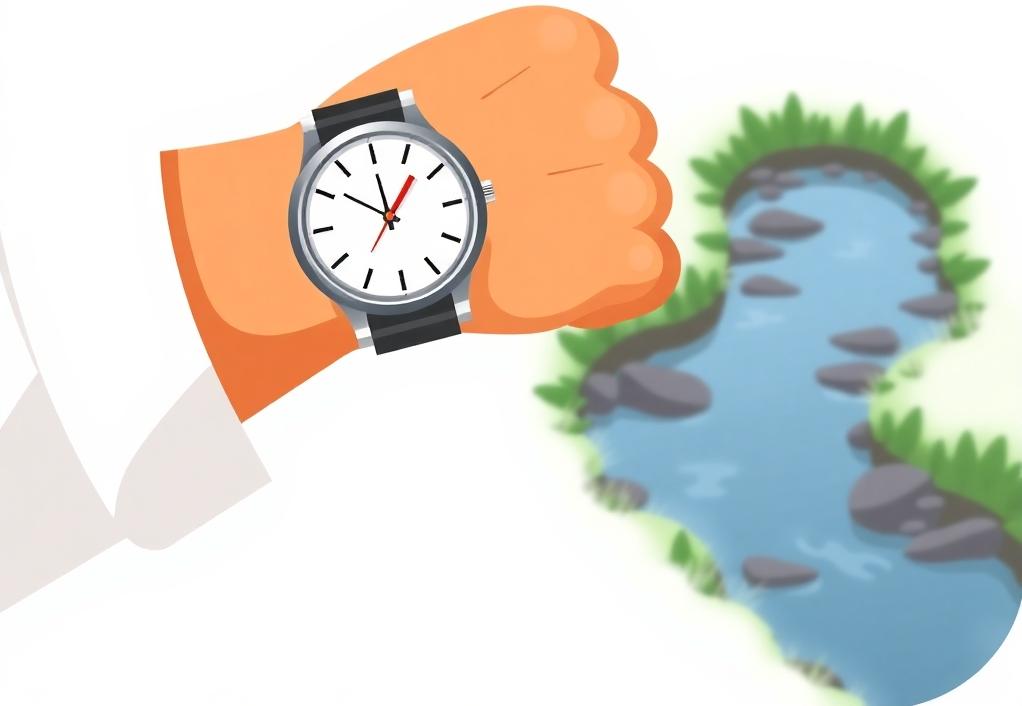
\includegraphics[height=\paperheight]{up_to_date.jpg}\hfil}\vfil}
		%https://www.flaticon.com/free-icon/decoration_2788716
		%<a href="https://www.flaticon.com/free-icons/decoration" title="decoration icons">Decoration icons created by Freepik - Flaticon</a>
		
	}
	\frame{
		\frametitle{Keeping your Community Up to Date}
		\begin{mdframed}[tikzsetting={draw=white,fill=white,fill opacity=0.8,
				line width=0pt},backgroundcolor=none,leftmargin=0,
			rightmargin=150,innertopmargin=4pt,roundcorner=10pt]
			\tableofcontents[currentsection,sections={1-4},hideothersubsections]
		\end{mdframed}
	}
}

%%%%%%%%%%%%%%%%%%%%%%%%%%%%%%%%%%%%%%%%%%%%%%%%%%%%%%%%%%%%%%%%%%%%%%%%%%%%%%%%
\begin{frame}
	\frametitle{Automated Social Media Posts - here: Mastodon}
	\begin{columns}
		\begin{column}{0.4\textwidth}
			
\includegraphics[width=0.7\textwidth]{bot.jpg}
			\vfil
			\only<2>{
\includegraphics[width=0.7\textwidth]{qrcode.png}}
		\end{column}
		\begin{column}{0.6\textwidth}
			Example post:\\
			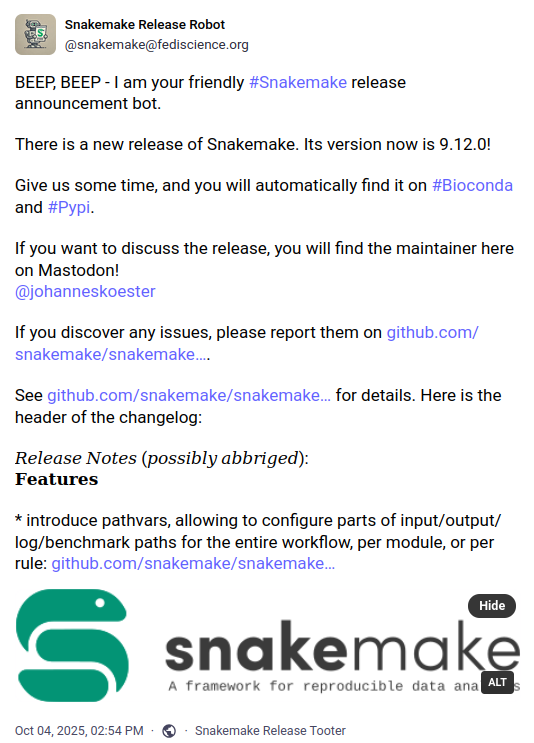
\includegraphics[width=0.7\textwidth]{snakemake_bot_post.png}
		\end{column}
	\end{columns}
\end{frame}

%%%%%%%%%%%%%%%%%%%%%%%%%%%%%%%%%%%%%%%%%%%%%%%%%%%%%%%%%%%%%%%%%%%%%%%%%%%%%%%%
\begin{frame}
	\frametitle{And if my Audience is not in the Fediverse?}
	Take a \lhref{https://github.com/defnull/fediwall}{fediwall} -- an appendix to a homepage, e.\,g.:
	
\end{frame}


%%%%%%%%%%%%%%%%%%%%%%%%%%%%%%%%%%%%%%%%%%%%%%%%%%%%%%%%%%%%%%%%%%%%%%%%%%%%%%%%
\begin{frame}[fragile]
	\frametitle{How does it work?}
	It uses a \lhref{https://github.com/snakemake/mastodon-release-post-action/}{special action}, key is the (Mastodon)-Secret:
	
			\begin{lstlisting}[language=yaml,basicstyle=\small\ttfamily\relax]
jobs:
  post_to_mastodon:
    if: "${{ contains(github.event.head_commit.message, 'chore(main): release') }}"
    runs-on: ubuntu-latest 
  steps: 
    - name: Checkout repository
      uses: actions/checkout@v4
    - name: Post to Mastodon
      uses: snakemake/mastodon-release-post-action@main 
      with:
        !access-token: ${{ secrets.MASTODONBOT }}!
		    \end{lstlisting}

\end{frame}





% \begin{frame}
%   \frametitle{List for possible further topics to cover}
%   \begin{itemize}
%   \item Something about data structures, e.g. a linked list, a tree, or something along
%     these lines
%   \item What is a good design? The Müller-script provides a really nice example!
%   \item Schlussthema: Some hints on programming -> file: XX\_hints.tex:
%     \begin{itemize}
%     \item Correctness first
%     \item Optimization second: quote from Donald Knuth
%     \item Some obvious optimizations: use constants or constexpr, loop unrolling, pure functions, load data continuously,\ldots
%     \end{itemize}
%   \end{itemize}
% \end{frame}







 
%%%%%%%%%%%%%%%%%%%%%%%%%%%%%%%%%%%%%%%%%%%%%%%%%%%%%%%%%%%%%%%%%%%%%%%%%%%%%%%% 
\begin{frame}<handout:0> 
  \frametitle{The End}
 \begin{center}
   \begin{figure}
     \centering
     
\includegraphics[width=0.7\textwidth]{the_end.jpg}
   \end{figure}
   Thank you for your attention! \newline Please give us some feedback!
 \end{center}
\end{frame}

\end{document}
